\documentclass[12pt, twoside]{article}
\usepackage[letterpaper, margin=1in, headsep=0.5in]{geometry}
\usepackage[english]{babel}
\usepackage[utf8]{inputenc}
\usepackage{amsmath}
\usepackage{amsfonts}
\usepackage{amssymb}
\usepackage{tikz}
\usetikzlibrary{quotes, angles}
\usepackage{graphicx}
\usepackage{enumitem}
\usepackage{multicol}

\newif\ifmeta
\metatrue %print standards and topics tags

\title{Regents Geometry}
\author{Chris Huson}
\date{February 2022}

\usepackage{fancyhdr}
\pagestyle{fancy}
\fancyhf{}
\renewcommand{\headrulewidth}{0pt} % disable the underline of the header
\raggedbottom

\fancyhead[LE]{\thepage}
\fancyhead[RO]{\thepage \\ Name: \hspace{4cm} \,\\}
\fancyhead[LO]{BECA / Dr. Huson / Geometry 7 Similarity}

\begin{document}

\subsubsection*{7.14 Exam: Similarity transformations}
I can solve problems using similarity criteria. \hfill CCSS.HSG.SRT.B.5
\begin{enumerate}
\begin{multicols}{2}
[\item A dilation maps triangle $PQR$ onto triangle $STU$ with $QR=7$ and $TU=14$.] \vspace{0.75cm}
  \begin{enumerate}
    \item $\overline{PR} \rightarrow$ \rule{2cm}{0.15mm}
    \item What scale factor maps\\
      $\triangle PQR \rightarrow \triangle STU$? \vspace{0.75cm}
    \item Given $PR=10$, find $SU$. \vspace{0.75cm}
    \item Given $ST=6$, find $PQ$.
    \end{enumerate}
    \begin{tikzpicture}[scale=0.9]
      \coordinate [label=above left:$P$](A) at (85:2);
      \coordinate [label=below:$Q$](B) at (0, 0);
      \coordinate [label=right:$R$](C) at (-20:3);
      \draw [thick] (A)--(B)--(C)--cycle;
      \draw [thick, xshift=2cm, yshift=2.5cm] (85:3) node[above]{$S$}--
      (0,0) node[below]{$T$}--
      (-20:4.5) node[right]{$U$}--cycle;
    \end{tikzpicture}
  \end{multicols}  \vspace{1cm}

\item Do Now: Given $\triangle PQR \sim \triangle STU$, $m\angle P=37^\circ$, and $m\angle T=46^\circ$. Find $m\angle Q$. \vspace{2cm}

\item $\triangle JKL$ with $J(-4,-2)$, $K(4,0)$, and $L(-2,4)$, is dilated  with a scale factor $k=1.5$ centered on the origin. Draw the image $\triangle J'K'L'$, labeling the vertices.
  \begin{center}
    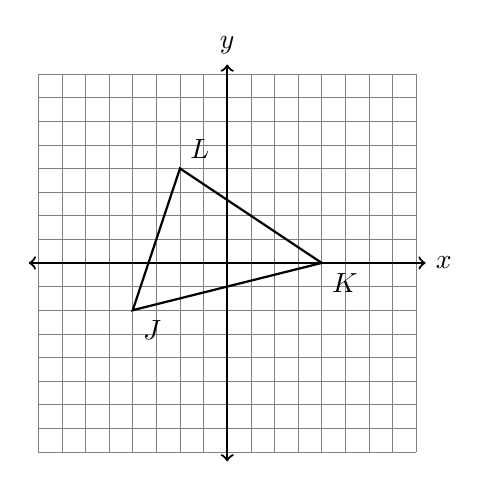
\begin{tikzpicture}[scale=.3]
      \draw [help lines] (-8,-8) grid (8,8);
      \draw [thick, <->] (-8.4,0) -- (8.4,0) node [right] {$x$};
      \draw [thick, <->] (0,-8.4)--(0,8.4) node [above] {$y$};
      \draw [thick]
      (-4,-2) node[below right] {$J$}--
      (4,0) node[below right] {$K$}--
      (-2,4) node[above right] {$L$}--
      cycle;
    \end{tikzpicture}
  \end{center}

\newpage
\item Triangle $ABC$ is dilated with a scale factor of $k$ centered at $A$, yielding $\triangle ADE$, as shown. Given $AB=10$, $BC=14$, $AC=16$, and $DE=21$. \\[0.25cm] Find $BD$, $AE$, and $k$ (the scale factor). \vspace{0.5cm}
\begin{center}
    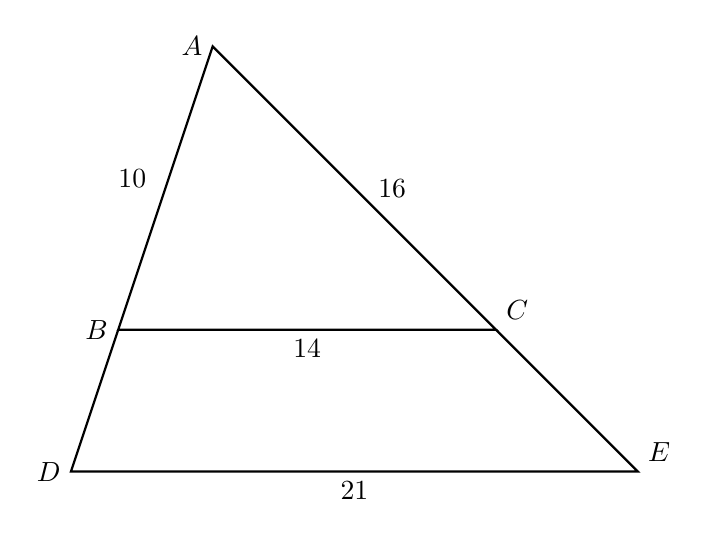
\begin{tikzpicture}[scale=0.6]
      \draw [thick]
      (0,0)node[left]{$B$}--
      (8,0)node[above right]{$C$}--
      (2,6)node[left]{$A$}--cycle;
      \draw [thick]
      (0,0)--
      (-1,-3)node[left]{$D$}--
      (11,-3)node[above right]{$E$}--(8,0);
      \node at (4,0)[below]{$14$};
      \node at (5.3, 3)[right]{$16$};
      \node at (0.3, 2.8)[above]{$10$};
      \node at (5,-3)[below]{$21$};
    \end{tikzpicture}
  \end{center}
\vspace{4cm}

\newpage

\item Given $\triangle ABP$ and $\triangle JKP$ as shown below. $\overline{AB} \parallel \overline{JK}$. $AP=5$, $JP=12$, and $JK=18$. Find $AB$.
\begin{center}
  \begin{tikzpicture}[scale=1.4]
      \draw [thick]
        (0.25,-1)node[right]{$B$}--
        (-0.5,2)node[left]{$K$}--
        (4,0)node[right]{$J$}--
        (0,0)node[above right]{$P$}--
        (-2,0)node[left]{$A$}--cycle;
    \end{tikzpicture}
    \end{center}
\vspace{2cm}


\begin{multicols}{2}[\item The diagram below shows $\triangle ABC$, with $\overline{AEB}$, $\overline{ADC}$, and $\angle ACB \cong \angle AED$. $AB=14$, $AD=8$, and $DE=4$.]
  \begin{enumerate}
    \item $\overline{AE} \rightarrow$ \rule{2cm}{0.15mm} \vspace{0.5cm}
    \item $\overline{AD} \rightarrow$ \rule{2cm}{0.15mm} \vspace{0.5cm}
    \item $\triangle ADE \sim$ \rule{2cm}{0.15mm} \vspace{0.5cm}
    \item What is the scale factor?\\[0.5cm] $k=$  \rule{2cm}{0.15mm}
    \item What is the length of $\overline{BC}$?
  \end{enumerate}
    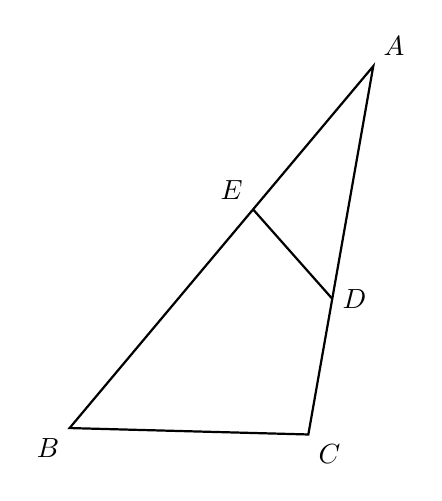
\begin{tikzpicture}%[scale=.48]
      \draw [thick]
      (0,0) node[above right] {$A$}--
      (230:6) node[below left] {$B$}--
      (260:4.75) node[below right] {$C$}--cycle;
      \draw [thick]
      (230:2.375) node[above left] {$E$}--
      (260:3) node[right] {$D$}--cycle;
    \end{tikzpicture}
  \end{multicols}

\newpage

  \item What is the smallest non-zero angle of rotation about its center that would map the pentagon onto itself? \vspace{0.25cm} %$ABCDE$
  \begin{center}
      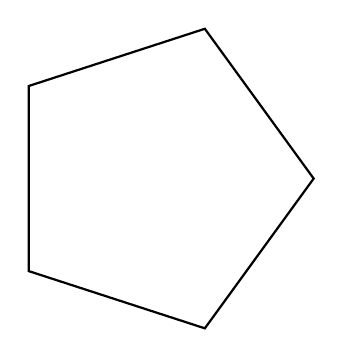
\begin{tikzpicture}%[scale=.48]
        \draw [thick]
        (0:2)--% node[right] {$A$}--
        (72:2)--% node[above right] {$B$}--
        (144:2)--% node[above left] {$C$} --
        (216:2)--% node[left] {$D$}--
        (288:2)--cycle;% node[right] {$E$}--cycle;
      \end{tikzpicture}
    \end{center} \vspace{0.5cm}

\item Triangle $ADE$ and its midline $\overline{BC}$ are drawn, with $B$ the midpoint of $\overline{AD}$ and $C$ the midpoint of $\overline{AE}$. The two medians $\overline{BE}$ and $\overline{CD}$ are drawn, as shown, intersecting in point $F$, the centroid.\\[0.25cm]
$\triangle FCB \sim \triangle FDE$ with scale factor $k=2$.\\[0.25cm]
Given $BC=9$, find $DE$. \\[0.25cm] Given $FE=12$, find $BF$. %\vspace{1cm}
\begin{center}
    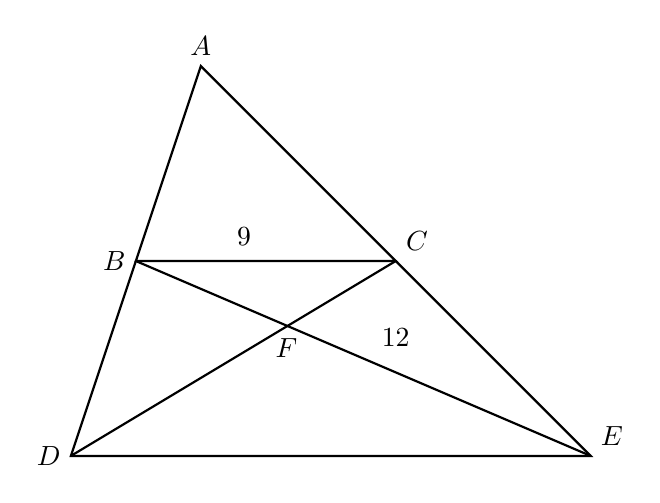
\begin{tikzpicture}[scale=0.55]
      \draw [thick]
      (0.5,1.5)node[left]{$B$}--
      (6.5,1.5)node[above right]{$C$}--
      (2,6)node[above]{$A$}--cycle;
      \draw [thick]
      (0.5,1.5)--
      (-1,-3)node[left]{$D$}--
      (11,-3)node[above right]{$E$}--(6.5,1.5);
      \draw [thick] (0.5,1.5)--(11,-3);
      \draw [thick] (6.5,1.5)--(-1,-3);
      \node at (3,2.5)[below]{$9$};
      \node at (3.5, -0.5)[right]{$F$};
      \node at (6.5, -.7)[above]{$12$};
      %\node at (-0.7, -1)[above]{$5$};
    \end{tikzpicture}
  \end{center} \vspace{1cm}


\item In the diagram below, the chords $\overline{AE}$ and $\overline{BD}$ intersect at $C$, with $\triangle ABC \sim \triangle DEC$, $BC=3$, $AC=4$, and $AE=11$. Determine the length of $\overline{CD}$.
    \begin{center}
    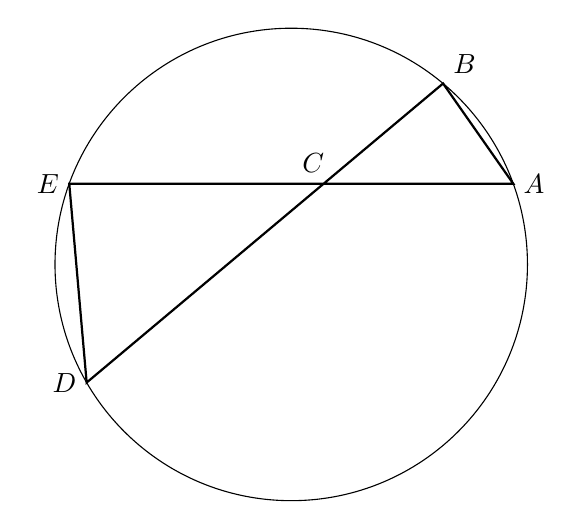
\begin{tikzpicture}[scale=.6]
      \draw (0,0) circle[radius=5];
      \draw [thick]
      (20:5) node[right] {$A$}--
      (160:5) node[left] {$E$}--
      (210:5) node[left] {$D$}--
      (50:5) node[above right] {$B$}--cycle;
      \draw (75:1.8) node[above] {$C$};
    \end{tikzpicture}
  \end{center}

\vspace{2cm}

\item In the diagram below, $\triangle ABC \sim \triangle DEF$, $DE=6$, $AB=x$, $AC=2x$, and $DF=2x+4$. Determine the length of $\overline{AB}$.
  \begin{center}
    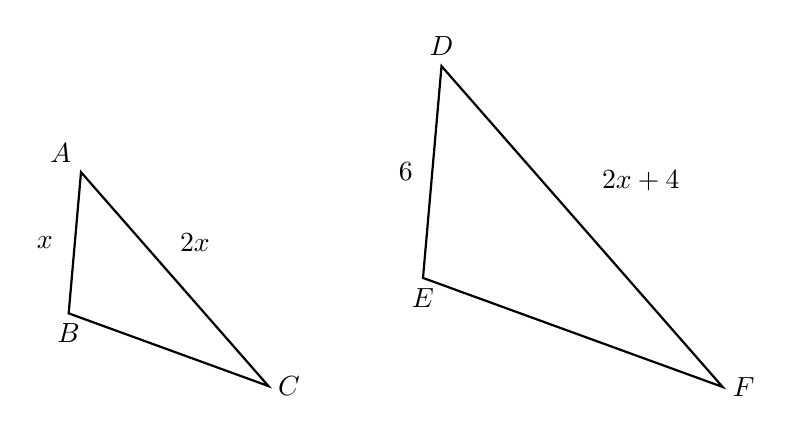
\begin{tikzpicture}[scale=0.9]
    \coordinate [label=above left:$A$](A) at (85:2);
    \coordinate [label=below:$B$](B) at (0, 0);
    \coordinate [label=right:$C$](C) at (-20:3);
      \draw [thick] (A)--(B)--(C)--cycle;
      \node at (95:1)[left]{$x$};
      \node at (35:1.75)[right]{$2x$};
      \draw [thick, xshift=5cm, yshift=0.5cm] (85:3) node[above]{$D$}--
      (0,0) node[below]{$E$}--
      (-20:4.5) node[right]{$F$}--cycle;
      \draw [thick, xshift=5cm, yshift=0.5cm](90:1.5) node[left]{$6$};
      \draw [thick, xshift=5cm, yshift=0.5cm](30:2.75) node[right]{$2x+4$};
  \end{tikzpicture}
  \end{center}

\end{enumerate}
\end{document}
